\documentclass{hw}
\usepackage[version=3]{mhchem}
\usepackage{nuc}
\usepackage{graphicx}
\usepackage{amsmath}
\usepackage{cancel}
\graphicspath{ {images/}}

\author{J.R. Powers-Luhn}
\date{2016/09/15}
\title{Homework \#3}

\begin{document}

\problem{}
	Compute the macroscopic fission cross section of 1, 2, 3, 4, and 5 wt\% enriched $ \ce{UO_2} $ with a density of $ 10.5g/cm^3 $. Use the $ 2200 m/s $ microscopic cross sections provided in Appendix A (pp. 606-610 in D\&H). What is the probability that a neutron will be absorbed in $ \ce{^{238}U} $ (relative to all absorptions) in these mixtures?
\solution

	$$ \Sigma_f = \cancel{N_{238} \sigma_f^{238}} + N_235 \sigma_f^{235} + \cancel{N_O \sigma_f^O}$$
	N is a number percentage--we must convert this from the provided weight percentage.
	\begin{align*}
		M(U) &= \frac{M(U-235) * M(U-238)}{wM(U-238)+(1-w)M(U-235)} \\
		N(U-235) &= \rho \frac{\frac{M(U)}{M(U-235)}w}{M(U-235)} A_V \\
	\end{align*}
	\begin{table}[h]
		\begin{tabular}{|c|c|c|}
			\hline
			w & N & $\Sigma_f $ \\
			\hline
			0.01 &  2.37135e+20 & 0.136827 \\
			0.02 & 4.74263e+20 & 0.27365 \\
			0.03 & 7.11384e+20 & 0.410469 \\
			0.04 & 9.48498e+20 & 0.547283 \\
			0.05 & 1.1856e+21 & 0.684094 \\
			\hline
		\end{tabular}
	\end{table}
	For the second part we must calculate $N(\ce{^{235}U})$.
	\begin{align*}
		N(U-238) &= \rho \frac{\frac{M(U)}{M(U-238)}(1-w)}{M(U-238)} A_V \\
		N(\ce{UO_2}) &= \rho \frac{A_V}{M(\ce{U)_2})}
	\end{align*}
	Results:
	\begin{table}[h]
		\begin{tabular}{|c|c|}
			\hline
			w & Probability \\
			\hline
			0.01 & 0.313432 \\
			0.02 & 0.310222 \\
			0.03 & 0.307013 \\
			0.04 & 0.303805 \\
			0.05 & 0.300598 \\
			\hline
		\end{tabular}
	\end{table}

\problem{}
	Using the Table of Nuclides at: http://atom.kaeri.re.kr/ton or that found at http://www.nndc.bnl.gov/sigma/ find the following information:
	\begin{enumerate}
		\item What is the total fission cross section of U-233, U-235, Pu-239, and Pu-241 at 0.0253 eV? 
		\item What is the accumulated fission yield of $ \ce{^{90}Sr} $ from the thermal fission of $ \ce{^{235}U} $?
		\item Obtain a plot of the $ \ce{^{241}Pu} $ total absorption cross section at 300K over the range $ 10^{-9} to 20 MeV $. Print out the plot and label the major features of the cross section behavior. Turn in the labeled plot.
	\end{enumerate}
\solution
	\part 
		\begin{table}[h]
			\begin{tabular}{ |c|c| }
				\hline
				Isotope & $ \sigma_f $ \\
				\hline
				$ \ce{^{233}U} $ & 532.707b \\
				$ \ce{^{233}U} $ & 585.472b \\
				$ \ce{^{233}U} $ & 751.322b \\
				$ \ce{^{233}U} $ & 1013.11b \\
				\hline
			\end{tabular}
		\end{table}
	\part $ 0.0578194 \pm 5.78194*10^{-4} $
	\part 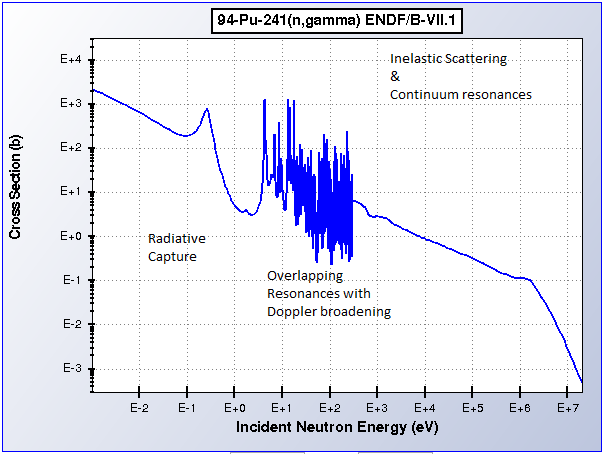
\includegraphics{ne470_03_02}
	

\problem{}
	How many collisions are required to slow down a neutron from 2MeV to 0.025 eV in 
	\begin{enumerate}
		\item Hydrogen,
		\item Deuterium,
		\item Graphite, and
		\item Lead?
	\end{enumerate}
\solution
	From Mragheb equation 37, we know that the average number of collisions required to slow a neutron from $ E $ to $ E' $ is:
	\[
		N = ln \left( \frac{E}{E'} \right) / \xi
	\]
	With values for $ \xi $ from Appendix A:
	\begin{table}[h]
		\begin{tabular}{ |c|c|c| }
			\hline
			Material & $ \xi $ & N \\
			\hline
			Hydrogen & 1.000 & 18.20 \\
			Deuterium & 0.725 & 25.1 \\
			Graphite & 0.158 & 115 \\
			Lead & 0.0096 & 1896 \\
			\hline
		\end{tabular}
	\end{table}

\problem{Duderstadt \& Hamilton, problem 3-8}
	Consider an infinitely large homogeneous mixture of $ \ce{^{235}U} $ and a moderating material. Determine the ratio of fuel-to-moderator density that will render this system critical for the following moderators: (a) graphite, (b) beryllium [\textit{sic}], (c) water ($ \ce{H_{2}O} $), and (d) heavy water ($ \ce{D_{2}O} $). Use the thermal cross section data given in Appendix A.
\solution
	From Appendix A:
	\begin{table}[h]
		\begin{tabular}{ |c|c|c| }
			\hline
			Moderator & $ \sigma_s $ (b) & $ \sigma_a $ (b) \\
			\hline
			$ Graphite $ & 4.8 & 0.004 \\
			$ Beryllium $ & 7.0 & 0.010 \\
			$ Water $ & 3.45 & 0.66 \\
			$ Heavy water $ & 0.449 & 0.001 \\
			\hline
		\end{tabular}
	\end{table}
	From Deuderstadt pg. 84, $ \eta $ and $ \epsilon $ change primarily with fuel selection and should be constant. For a homogeneous core, the fast fission factor, $ \epsilon $ is approximately 1 \footnote{http://www.nuclear-power.net/nuclear-power/reactor-physics/nuclear-fission-chain-reaction/fast-fission-factor/}. To calculate a value for $ \eta $ (neglecting neutron re-emission reactions) we use the equation:
	\begin{align*}
		\eta_{\ce{^{235}U}} &= v * \frac{\sigma_f}{\sigma_f + \sigma_{\gamma}} \\
		&= 2.068
	\end{align*}
	We can also say that all neutrons are successfully thermalized, meaning $p=1$. We then set Deuderstadt equation 3-13 to 1.0:
	\begin{align*}
		k_{\inf} &= \eta_{\ce{^{235}U}} f = 1.0 \\
		1 / \eta_{\ce{^{235}U}} &= f \\
		1 / \eta_{\ce{^{235}U}} &= \frac{N_{F} \sigma^{F}_a}{N_{F}\sigma^{F}_a + N_{M} \sigma^M_a} \\
		1 / \eta_{\ce{^{235}U}} * \left( N_{F}\sigma^{F}_a + N_{M} \sigma^M_a \right) &= N_{F} \sigma^{F}_a \\
		\frac{N_M}{N_F} &= \left( \eta - 1 \right) \frac{\sigma^F_a}{\sigma^M_a}
	\end{align*}
	\begin{table}[h]
		\begin{tabular}{ |c|c| }
			\hline
			Moderator & Moderator/Fuel Number Ratio \\
			\hline
			Water & 12.43 \\
			Heavy Water & 8202 \\
			Graphite (C) & 2050 \\
			Beryllium & 820.2 \\
			\hline
		\end{tabular}
	\end{table}

\problem{Duderstadt \& Hamilton, problem 3-1}
	What is the maximum value of the multiplication factor that can be achieved in any conceivable reactor design?
\solution
	We know that the multiplication factor for a thermal reactor core is: \[ k_{eff} = \epsilon p f \eta P_{FNL} P_{TNL} \]

	We can assume that an ideal core would be large enough to allow for no leakage, so $ P_{fast non leakage} = P_{thermal non leakage} = 1 $. If we assume 100\% enrichment, p = $ \epsilon $ = 1.0. Finally we should maximize $ \eta $. For thermal fuels, from the appendix A data:
	\begin{table}[h]
		\begin{tabular}{|c|c|c|c|c|}
			\hline
			Fuel & $\sigma_{\gamma}$ & $\sigma_f$ & v & $\eta$ \\
			\hline
			U-233 & 49 & 524 & 2.4968 & 2.2832 \\
			U-235 & 101 & 577 & 2.4355 & 2.0726 \\
			Pu-239 & 274 & 741 & 2.88 & 2.1025 \\
			Pu-241 & 425 & 950 & 2.9479 & 2.0367 \\
			\hline
		\end{tabular}
	\end{table}
	This table assumes only thermal fuels, so we will need a moderator. Our concern here is to avoid absorption by the fuel, so we should select a moderator with a high $ \Sigma_s $ and low $ \Sigma_a $. We would also want a large $\xi$ to minimize the number of possibilities for absorption. This is captured in the moderating ratio, for which heavy water has the highest value (5670).

	This only considers thermal fuels. A fast fuel would not require a moderator, meaning $f=1$, but might have a poor value of $\eta$, making it unsuitable.

	Actual reactor design would require values of k very close to 1 in order to allow for reactor control. If we assume a core has a neutron generation time on the order of a millisecond, a k value of 1.0093 means power will go from 1\% to exceeding design capacity in less than 0.5 seconds. This provides very little time for human feedback. Even if we assume that automated controls are an order of magnitude faster, this still only allows for a k value of 1.096 before exceeding design capacity.

\end{document}